\documentclass[10pt]{mypackage}

\usepackage{mlmodern}
%\usepackage{newpxtext,eulerpx,eucal}
%\renewcommand*{\mathbb}[1]{\varmathbb{#1}}

\usepackage{homework}
%\usepackage{notes}

%\usepackage[ backend=bibtex, style = alphabetic, sorting=ynt ]{biblatex}
%\addbibresource{  }

\usepackage{parskip}

\fancyhf{}
\fancyhead[R]{Avinash Iyer}
\fancyhead[L]{Algebraic Topology: Homework 3}
\fancyfoot[C]{\thepage}

\setcounter{secnumdepth}{0}

\begin{document}
\RaggedRight
\begin{problem}[Problem 1]
  Prove that our cell complex structure for $T^2$ coincides with a product cell complex structure on $S^1\times S^1$ for some cell complex structure on $S^1$.
\end{problem}
\begin{solution}
  We consider the cell complex structure on $S^1$ given by one $0$-cell and one $1$-cell with characteristic map $\Phi\colon [0,1]\hookrightarrow S^1$ identifying $0\sim 1$. If we consider two copies of $S^1$ in this fashion, this gives rise to a CW complex structure with
  \begin{itemize}
    \item $1$ $0$-cell, which we label as $e^0$;
    \item $2$ $1$-cells, which we label as $e^1_1$ and $e^1_2$;
    \item and $1$ $2$-cell, which we label as $e^2$.
  \end{itemize}
  Since the attaching maps (viewed as restrictions of the characteristic maps at the boundary) for both $e^1_1$ and $e^1_2$ coincide at $e^0$, it follows that there are characteristic maps $\Phi_{1,2}|_{\partial e^1_{1,2}} = e^0$
  \begin{align*}
    \Phi_{1,2}\colon e^1_{1,2}\hookrightarrow S^1\times S^1
  \end{align*}
  such that
  \begin{align*}
    \Phi_{1,2}|_{\partial e^1_{1,2}}\left( \partial e^{1}_{1,2} \right) = e^0.
  \end{align*}
  Therefore, we may draw the $1$-skeleton as the following identification.
  \begin{center}
    \begin{tikzpicture}
    % Define vertices
    \coordinate (v1) at (0,3);
    \coordinate (v2) at (3,3);
    \coordinate (v3) at (3,0);

    % Draw edges
    \draw[very thick] (v1) -- (v2);
    \draw[very thick] (v2) -- (v3);

    % Draw vertices as filled dots
    \fill (v1) circle (3pt);
    \fill (v2) circle (3pt);
    \fill (v3) circle (3pt);

    % Labels for vertices
    \node at (-0.3,3) {$e_0$};
    \node at (3,3.3) {$e_0$};
    \node at (3,-0.3) {$e_0$};

    % Labels for edges
    \node at (1.5,3.3) {$e_1^1$};
    \node at (3.4,1.5) {$e_2^1$};

    \end{tikzpicture}
  \end{center}
  We consider the $2$-cell $e^2$ as a square given by $e^1_1\times e^1_2$. That is, it is given by the following diagram.
  \begin{center}
    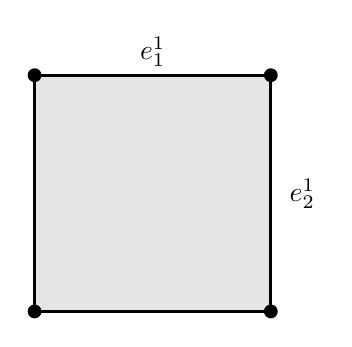
\begin{tikzpicture}
  % Define vertices
  \coordinate (v1) at (0,0);
  \coordinate (v2) at (3,0);
  \coordinate (v3) at (3,3);
  \coordinate (v4) at (0,3);

  % Draw filled square with light gray shading
  \fill[gray!20] (v1) -- (v2) -- (v3) -- (v4) -- cycle;
  % Draw edges
  \draw[very thick] (v1) -- (v2) -- (v3) -- (v4) -- cycle;

  % Draw vertices as filled dots
  \fill (v1) circle (2.5pt);
  \fill (v2) circle (2.5pt);
  \fill (v3) circle (2.5pt);
  \fill (v4) circle (2.5pt);

  % Labels for edges
  \node at (1.5,3.3) {$e_1^1$};
  \node at (3.4,1.5) {$e_2^1$};

\end{tikzpicture}
  \end{center}
  We observe that the characteristic map for $e^2$, $\Psi\colon e^2\hookrightarrow S^1\times S^1$, is such that $\partial e^2$ is identified with the $1$-skeleton. Therefore, we obtain the following diagram.
  \begin{center}

    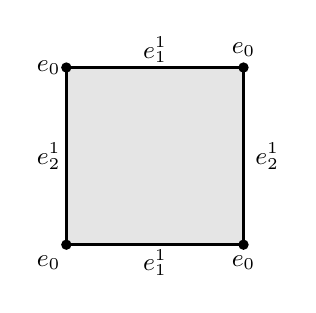
\begin{tikzpicture}[scale=0.75]
  % Define vertices
  \coordinate (v1) at (0,0);
  \coordinate (v2) at (3,0);
  \coordinate (v3) at (3,3);
  \coordinate (v4) at (0,3);

  % Draw filled square with light gray shading
  \fill[gray!20] (v1) -- (v2) -- (v3) -- (v4) -- cycle;
  % Draw edges
  \draw[very thick] (v1) -- (v2) -- (v3) -- (v4) -- cycle;

  % Draw vertices as filled dots
  \fill (v1) circle (2.5pt);
  \fill (v2) circle (2.5pt);
  \fill (v3) circle (2.5pt);
  \fill (v4) circle (2.5pt);

  % Labels for edges
  \node at (1.5,3.3) {\small $e_1^1$};
  \node at (3.4,1.5) {\small $e_2^1$};
  \node at (-0.3,3) {\small $e_0$};
  \node at (3,3.3) {\small $e_0$};
  \node at (3,-0.3) {\small $e_0$};
  \node at (-0.3,-0.3) {\small $e_0$};
  \node at (1.5,-0.3) { \small $e_1^1$ };
  \node at (-0.3,1.5) { \small $e_2^1$ };
\end{tikzpicture}
  \end{center}
  This is precisely the cell complex structure of the torus.
\end{solution}
\begin{problem}[Problem 2]
  Prove that if $X$ is a cell complex, then so is the suspension $SX$.
\end{problem}
\begin{solution}
  We observe that the product $X\times [0,1]$ is a cell complex as it is a Cartesian product of a cell complex with one $1$-cell, $e^1 \cong [0,1]$, and two $0$-cells, which are the endpoints of the interval. Similarly, $X\times \set{0}$ and $X\times \set{1}$ are cell complexes as they are the Cartesian product of a cell complex with the $0$-cell, $e^0 \cong \set{0} = \set{1}$.

  Since $X\times \set{0}$ is a subcomplex of $X\times [0,1]$ with the attaching map given by restricting the product to $\set{0}$, it follows that $X\times [0,1]/\left( X\times \set{0} \right)$ is a cell complex, so $SX = X\times [0,1]/\left( X\times \set{0} \right)/\left( X\times \set{1} \right)$ is a cell complex.
\end{solution}
\begin{problem}[Problem 3]
  Consider the infinite-dimensional sphere $S^{\infty} = \bigcup_{n}S^n$, given by attaching two cells of arbitrarily high dimension.
  \begin{enumerate}[(a)]
    \item Describe all the subcomplexes of $S^{\infty}$ with this cell complex structure.
    \item Prove that $S^{\infty}$ is contractible.
  \end{enumerate}
\end{problem}
\begin{solution}\hfill
  \begin{enumerate}[(a)]
    \item The $n$-skeleton for $X$ is given by
      \begin{align*}
        X^{n} &= 2e^{n}\cup 2e^{n-1}\cup\cdots\cup 2e^{1}\cup 2e^{0},
      \end{align*}
      where we let $e^{i}$ represent the $i$-cell. Each of the $n$-skeleta is a subcomplex of $S^{\infty}$. Additionally, we observe that within the $n$-skeleton, the attaching maps for each $e^n$ have it such that $\partial e^n$ is identified with $X^{n-1}$, so there are two sub-skeleta defined by
      \begin{align*}
        A_1 &= e^n\cup 2e^{n-1}\cup \cdots\cup 2e^1 \cup 2e^0\\
        A_2 &= e^n\cup 2e^{n-1}\cup \cdots\cup 2e^1 \cup 2e^0.
      \end{align*}
      This holds for each $n$-skeleton, so these are the subcomplexes of $S^{\infty}$.
  \end{enumerate}
\end{solution}

\end{document}
